\documentclass[a4paper, 12pt]{article}
\usepackage{comment} % enables the use of multi-line comments (\ifx \fi) 
\usepackage{lipsum} %This package just generates Lorem Ipsum filler text. 
\usepackage{fullpage} % changes the margin
\usepackage{graphicx}
\usepackage{epsfig}
\usepackage{listings}
\usepackage{xcolor}
\lstset { %
	language=C++,
	backgroundcolor=\color{black!5}, % set backgroundcolor
	basicstyle=\footnotesize,% basic font setting
}

\begin{document}
%Header-Make sure you update this information!!!!
\noindent
\large\textbf{Lab 4 Report} \hfill \textbf{Abhishek Srivastava} \\
\normalsize CS260-001: Computer Security \hfill Student Id: 861307778 \\
\normalsize Prof. Heng Yin \hfill \today \\
\hrule

\section*{Experimenting with Evolutionary Fuzzing}

\textbf{Problem 1}

Does AFL crash the program? Explain why do you think AFL can or cannot crash it?\\

\noindent
\textbf{Solution}

Yes, the AFL program does crashes both of the program ran with it and it generated 3 unique crashes and covered 14 total control paths as well for each case. AFL is fuzzing tool and it generates different test cases based on the seeded file which is being provided initially. The main focus of AFL is to generate such cases so that it can cover as many possible paths as possible in the program. It applies multiple kind of operation on the input test case such as: \textbf{flip1}, \textbf{havoc}, \textbf{arith8} and \textbf{slice} to generate fuzzy inputs and observe how program behaves.\\


 
Figure 1 and Figure 2 shows the result of running AFL for about 10 mins.

\begin{figure}[!b]
	\centering
	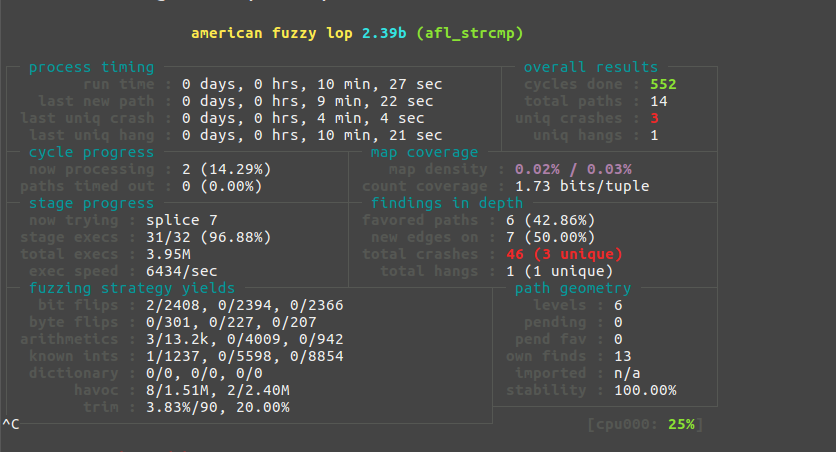
\epsfig{file=Lab_4_SS1.png, height=4in, width=7in}
	\caption{Screen Shot of running AFL for program afl\_strcmp.}
\end{figure}

\begin{figure}
	\centering
	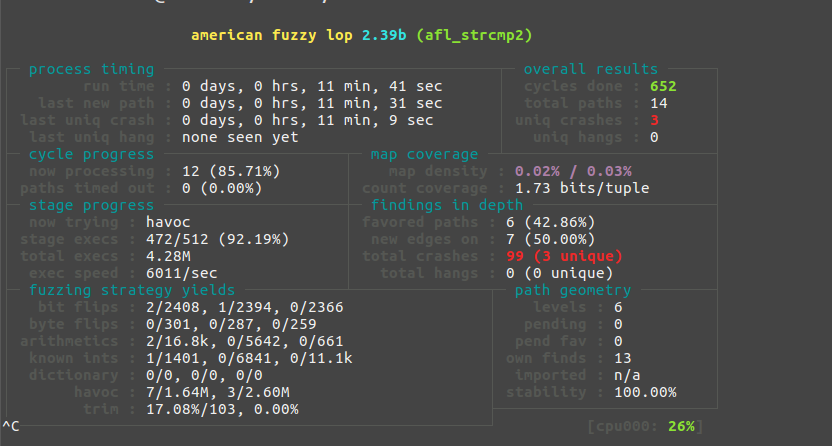
\epsfig{file=Lab_4_SS2.png, height=4in, width=7in}
	\caption{Screen Shot of running AFL for program afl\_strcmp2.}
\end{figure}

\newpage
\noindent
\textbf{Problem 2}

Look at the seed files (ending with +cov) in the queue. These inputs increase the branch coverage according to AFL. For each of these seeds, explain what branch coverage it causes. You can use the Line numbers in the source file.\\

\noindent
\textbf{Solution}

\textbf{afl\_strcmp}: Figure 3 shows the source code of the programs taken as reference for line numbers. Original Text was : ``abABcdCD". Table 1 shows the seed file names, their content and their branch coverage. I am not considering while loop to take input as a branch. Also some coverage path are coming as same because I am not including the loop repetition over the same branch. Branch at 12 takes two routes so different routes will generate different coverage. I have marked the arrows to show what branches are covered at what line number.
\begin{table}[h]
	\centering
	\caption{Output of seed files for test afl\_strcmp file.}
	\begin{tabular}{|c|c|l|} \hline
		Seed Name&Seed Input&Branch Coverage\\ \hline
		id:000001,src:000000,op:flip1,pos:0,+cov&cbABcdCD&30\rightarrow9\rightarrow12\rightarrow40\\ \hline
		id:000007,src:000000,op:havoc,rep:16,+cov&d\^S\^\@\^D\^@\^F\^@\^A\^Ad&30\rightarrow12\rightarrow40\\ \hline
		id:000009,src:000001,op:arith8,pos:1,val:+17,+cov&csABcdCD&30\rightarrow9\rightarrow12\rightarrow40\\ \hline
		id:000010,src:000009,op:arith8,pos:2,val:-19,+cov&cs.BcdCD&30\rightarrow9\rightarrow10\rightarrow34\rightarrow12\\ \hline
		id:000012,src:000010,op:havoc,rep:2,+cov&cs.ucdCD&30\rightarrow9\rightarrow10\rightarrow34\rightarrow9\rightarrow12\\ \hline
		id:000013,src:000012,op:flip1,pos:4,+cov&cs.u?dCD&30\rightarrow9\rightarrow10\rightarrow34\rightarrow9\rightarrow12\\ \hline
	\end{tabular}
\end{table}
\begin{figure}
	\centering
	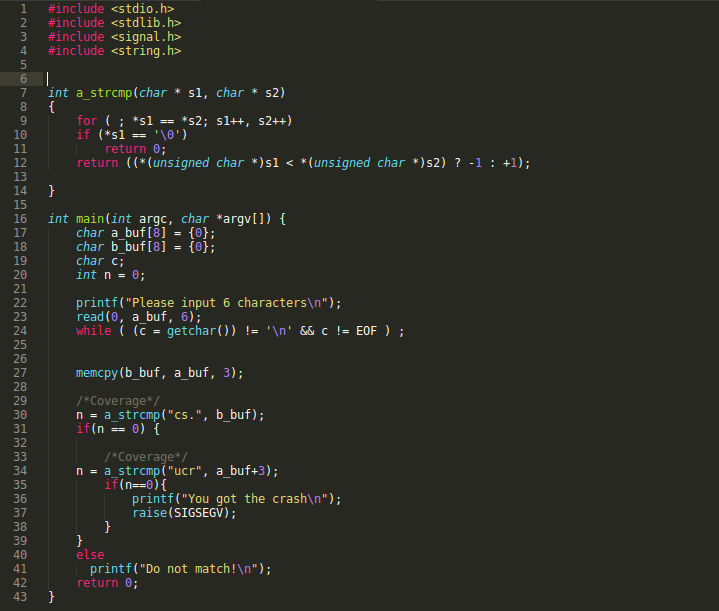
\epsfig{file=Lab_4_SS3.png, height=7.5in, width=7in}
	\caption{ Code for the program afl\_strcmp.}
\end{figure}
\newpage
\textbf{afl\_strcmp2}: Figure 4 shows the source code of the program taken as reference for line numbers. Original Text input was : ``abABcdCD". Table 2 shows the seed file names, their content and there branch coverage. I have taken same assumptions as the previous program. Branch at 12 and 21 takes two routes so different routes will generate different coverage.
\begin{table}[h]
	\centering
	\caption{Output of seed files for test afl\_strcmp2 file.}
	\begin{tabular}{|c|c|l|} \hline
		Seed Name&Seed Input&Branch Coverage\\ \hline
		id:000001,src:000000,op:flip1,pos:0,+cov&cbABcdCD&39\rightarrow9\rightarrow12\rightarrow49\\ \hline
		id:000008,src:000000,op:havoc,rep:64,+cov&Gúè^@ú^@ùùú[[^@dùú&39\rightarrow12\rightarrow49\\ \hline
		id:000009,src:000001,op:arith8,pos:1,val:+17,+cov&csABcdCD&39\rightarrow9\rightarrow12\rightarrow49\\ \hline
		id:000010,src:000009,op:arith8,pos:2,val:-19,+cov&cs.BcdCD&39\rightarrow9\rightarrow10\rightarrow43\rightarrow21\\ \hline
		id:000012,src:000010+000002,op:splice,rep:2,+cov&cs.u??&39\rightarrow9\rightarrow10\rightarrow43\rightarrow18\rightarrow21\\ \hline
		id:000013,src:000012,op:havoc,rep:2,+cov&cs.ucs?u&39\rightarrow9\rightarrow10\rightarrow43\rightarrow18\rightarrow21\\ \hline
	\end{tabular}
\end{table}
\begin{figure}
	\centering
	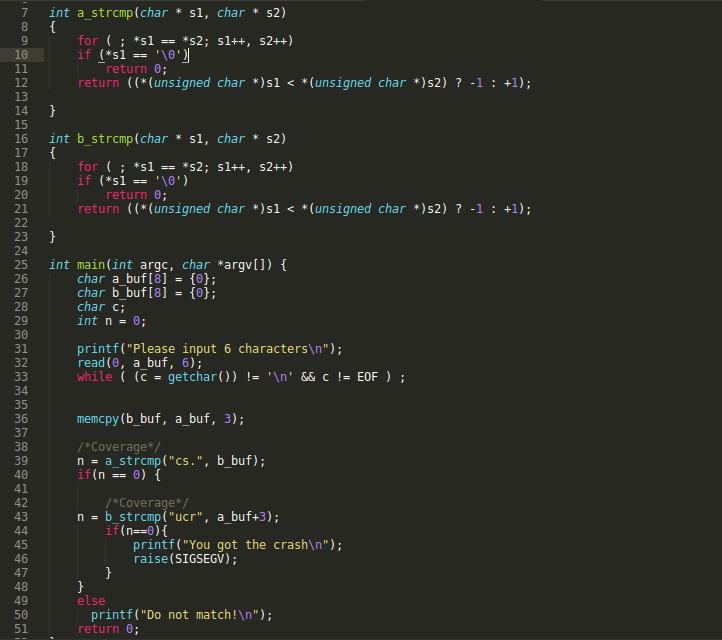
\epsfig{file=Lab_4_SS4.png, height=7.5in, width=7in}
	\caption{ Code for the program afl\_strcmp2.}
\end{figure}

\newpage
\noindent
\textbf{Problem 3}

Pay attention the file names, they show how these inputs are mutated from their parents. Please explain the evolution of these seed files.\\

\noindent
\textbf{Solution}

Each seed file follow the some pattern to generate the names for fuzzed inputs file names. \\

The original input name for (\textbf{id:000000,orig:test.txt}).  \textbf{id} means seed id for this file is 000000,  \textbf{orig} indicates that it is original file input and its name is \emph{test.txt}.\\

For the seeded file name are like (\textbf{id:000013,src:000012,op:havoc,rep:2,+cov}). \textbf{id} means the seed id for this file is 000013, \textbf{src} means the source file id for generating this file is 000012, \textbf{op} means which operation it performed on the source file to generate the seed file. \textbf{rep} this field is operation dependent here it means number of repetitions done. \textbf{+cov} means it has performed additional coverage.
   
\end{document}
